\chapter{مقدمه، تعریف مساله، راه‌ حل پیشنهادی}
\section{مقدمه}
 با ظهور کامپیوتر و علم رایانه بازارهاي مالی  جهان به سمت الکترونیکی شدن پیش رفتند. امروزه تقریبا تمام بازارهاي مالی و
حتی گاهی غیرمالی در بستر کامپیوتري و هوشمند فعال هستند تا جایی که بازارهایی مانند نزدک\LTRfootnote{\lr{NASDAQ}} یا بازارهاي مربوط به  رمزارزها\LTRfootnote{Cryptocurrency} تنها در این بسترها قابل دسترسی می‌باشند و هیچ مکان فیزیکی‌اي براي مبادله درون این بازارها وجود ندارد.\\
تعداد زیادي از فعالان اقتصادي در این بازارها فعالیت روزانه خود را دنبال می‌کنند که محور اصلی فعالیت آن‌ها پیش‌بینی ویژگی‌های مختلف بازار مانند قیمت دارایی‌ها، میزان ریسک سرمایه گذاری در یک دارایی، تغییرات و نوسان تغییرات قیمت است. اما همان طور که انتظار می‌رود این زمینه نیز از پیشرفت هوش مصنوعی بی‌نصیب نمانده‌است و دستخوش تغییرات زیادي شده است. یکی از این تغییرات به وجود آمدن عوامل خودکار خرید و فروش است. عوامل هوشمندي که با تکیه بر ابزارها و روش‌هاي از پیش تعیین شده اقدام به خرید و فروش در این بازارها می‌کنند. پیش‌بینی سری‌های زمانی نقشی کلیدی در فعالیت تمامی این عوامل دارد، که باعث شده است مطالعات گسترده‌ای بر روی سری‌های زمانی مالی صورت بگیرد.\\
از ویژگی‌هایی که همواره مورد توجه فعالان این بازارها بوده است محاسبه و پیش‌بینی میزان نوسان قیمت و نه خود آن در بازارهاي مالی در بازه‌هاي زمانی مشخص می‌باشد. داشتن تخمینی از نوسان آینده‌ی بازار و همینطور میزان تغییرات قیمت در ساعات آینده می‌تواند استراتژي‌هاي خرید و فروش هر عاملی، خواه هوشمند و خواه انسانی، را به کلی دستخوش تغییر کند. علاوه بر آن، نوسان یک دارایی از اهمیت بسیاري در جهت محاسبه‌ي سود و امکان واگذاري اوراق بهادار مشتقه‌ی آن برخوردار است. از این رو تحقیقات زیادي در مورد تخمین میزان نوسانات بازارهاي مالی انجام شده است که هر یک سعی کرده‌اند از منابع داده‌ي گوناگون، از تغییرات قیمت تا کامنت‌هاي شبکه‌هاي اجتماعی استفاده کنند.
\section{تعریف مساله}
\subsection{رمزارزها}
ارز دیجیتال یا رمزارز نوعی پول مجازي است که از فناوري رمزنگاري استفاده می‌کند و معمولاً به صورت غیرمتمرکز اداره می‌شود. رمزارزها میتوانند مانند سایر ارزهاي بدون پشتوانه برای مبادله، انجام تراکنش، خرید آنلاین و ... مورد استفاده قرار بگیرند.\\
بیتکوین\LTRfootnote{Bitcoin} اولین پیاده سازی موجود از این رمزارز‌هاست که هم اکنون از بیشترین ارزش بازار در میان تمامی رمزارزها برخوردار است\cite{nakamoto2008bitcoin}. بیتکوین بدون مدیریت مرکزی عمل می‌کند و از طریق اینترنت و تکنولوژی شبکه‌ی بلوکی\LTRfootnote{Blockchain} خود پرداخت‌های بین کاربران را ذخیره و تایید می‌کند. هر پرداخت جدید به وسیله‌ی بیت کوین باید به اطلاع شبکه‌ی موجود رسانده شود و یک گزارش از آن در زنجیره‌ی بلوکی بیتکوین ذخیره شود. برای تایید و ذخیره شدن در زنجیره‌ی بلوکی اصلی، تراکنش‌ها باید توسط رایانه‌هایی که وظیفه‌ی تایید تراکنش‌ها را دارند تایید شوند. این رایانه‌ها استخراج‌کننده\LTRfootnote{Miner} نامیده می‌شوند و در ازای عملیات تایید مقداری بیتکوین به عنوان پاداش دریافت می‌کنند.\\
علاوه بر انتقال مستقیم بیتکوین در زنجیره‌ی بلوکی،‌مبادله‌ي بیتکوین و دیگر رمزارزها در صرافی‌های آنلاین نیز صورت می‌گیرد. دفتر سفارشات\LTRfootnote{Order book} داده ساختاریست که در این صرافی‌ها نگهداری می‌شود و شامل سفارشات خرید و فروش است\cite{naes2006order}.
\begin{figure}[!t]
	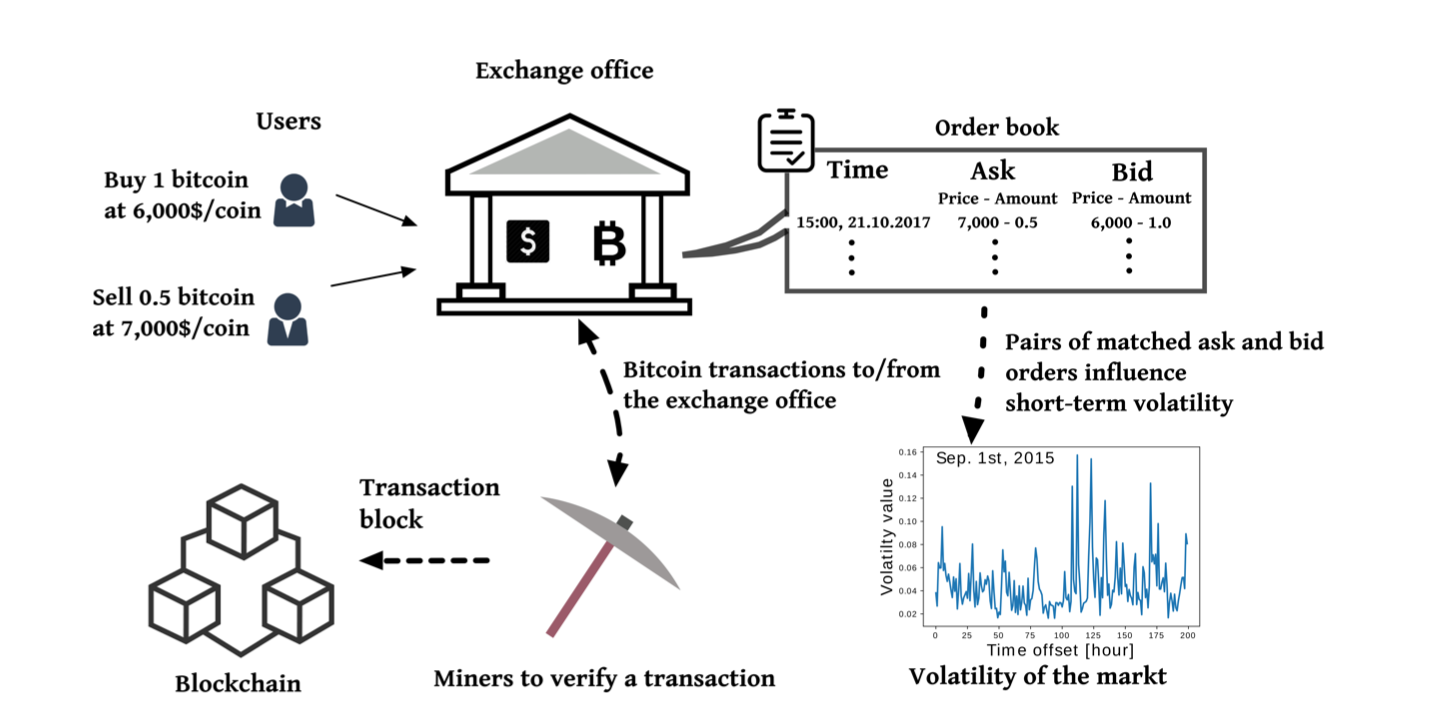
\includegraphics[width=0.6 \textwidth]{images/mine}
	\centering
	\caption{روند کلی استخراج و نحوه‌ی کار رمز‌ارزها \cite{guo2018bitcoin}.
	}
	\label{fig.panjda}
\end{figure}

\subsection{دفتر سفارشات}
دفتر سفارشات داده ساختاریست که نگهدارنده‌ي وضعیت فعلی بازار و سفارشات خریداران و فروشندگان است. هر سفارش خرید\LTRfootnote{bid} شامل دو عدد حجم و قیمت است، که بیان کننده‌ی تقاضای خرید به مقدار حجم مشخص‌شده از آن دارایی در قیمتی کمتر یا مساوی با قیمت مشخص شده‌اند. در مقابل هر تقاضای فروش\LTRfootnote{ask} نیز نشان دهنده‌ی تقاضای فروش به مقدار حجم مشخص‌شده از آن دارایی در قیمتی بیشتر و یا مساوی با قیمت مشخص شده است. معامله و جابه‌جایی دارایی تنها هنگامی صورت می‌گیرد که قیمت پیشنهادی خریدار بیشتر و یا مساوی با قیمت پیشنهادی فروشنده باشد، در چنین شرایطی به میزان حجم مشخص شده از دارایی فروشنده به دارایی خریدار انتقال صورت می‌گیرد و هر دو سفارش از دفتر سفارشات خارج می‌شوند.
\begin{figure}[!t]
	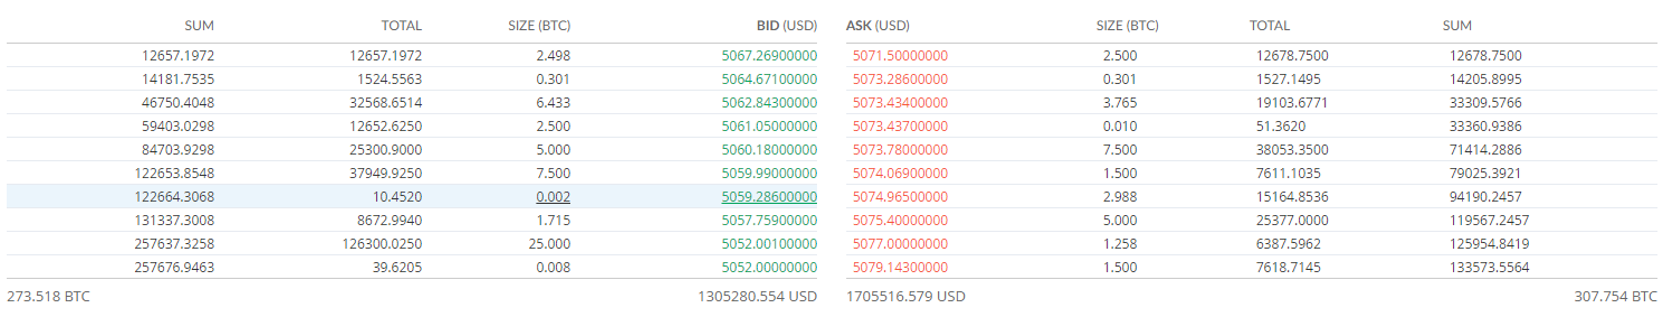
\includegraphics[width=1.0 \textwidth]{images/orderbook}
	\centering
	\caption{ نمونه‌ای از دفتر سفارشات مربوط به بیتکوین.
	}
	\label{fig.panda}
\end{figure}
\subsection{نوسان قیمت در رمزارزها}
به دلیل استقبال گسترده از رمزارزها در سال‌های گذشته، مطالعات زیادی بر روی ویژگی‌های آماری بازار رمزارز‌های مختلف انجام شده است. یکی از زمینه‌های اصلی این مطالعات نوسان قیمت در این بازارها بوده‌است. بر خلاف افزایش اندازه بازار رمزارز‌ها، این بازارها همچنان دارای نوسان بسیار زیادی نسبت به بازار‌های هم اندازه‌ هستند که محل بررسی بوده است\cite{katsiampa2017volatility}. برخی این میزان از نوسان را به دلیل عدم وجود روش دقیقی برای ارزش‌گذاری این ارزها که مورد پذیرش همگان باشد می‌دانند. این مسئله موجب شده است تا مطالعات مختلفی به بررسی این ویژگی این بازارها بپردازند.
\section{راه حل پیشنهادي}
در این پروژه، سعی داریم تا با استفاده از اطلاعات موجود در دفتر سفارشات یک مدل نوسانی بر پایه یادگیری عمیق ارائه بدهیم. مطالعات مختلفی نشان دهنده‌ی اهمیت و تاثیر دفتر سفارشات بر متغیر‌های مختلف بازارها بوده‌اند. در مقایسه با دیگر منابع داده‌ی موجود، دفتر سفارشات حجیم‌تر است و شامل اطلاعات جزئی‌تری از وضعیت فعلی بازار است. این اطلاعات که شامل سفارشات انجام نشده هستند تا حدودی خبر از آینده‌ی نزدیک بازار می‌دهند، و از این جهت در مقدار و جهت تغییرات بازار که همان نوسان است تاثیر قابل توجهی دارند\cite{guo2018bitcoin}و\cite{donier2015markets}.\\
از طرفی شبکه‌های عصبی در سال‌های گذشته در بسیاری از زمینه‌ها به صورت گسترده به کار گرفته شده‌اند و نتایج بسیار امیدوار کننده‌ای ارائه داده‌اند. با این وجود، شبکه‌های عصبی معمولی در استفاده از دنباله‌ی طولانی‌ای از داده‌های ورودی و یادگیری در چنین شرایطی مشکلات مختلفی دارند و کارا نیستند\cite{wang2015back}. در این میان، شبکه‌های عصبی بازگشتی\LTRfootnote{Recurrent Neural Network}، به کمک طراحی خود و استفاده از دنباله‌ای از اطلاعات ورودی برای پیش‌بینی اطلاعات آینده، عملکرد بهتری در این زمینه‌ ارائه کرده‌اند. هرچند که این مدل‌ها نیز در یافتن و استفاده از اطلاعات بلندمدت در دنباله‌ی طولانی از اطلاعات ناتوانند. شبکه‌های بازگشتی معمولی در مواجهه با دنباله‌ی طولانی از اطلاعات ،به ویژه در مسائل سری‌های زمانی، با مشکل ناپدید شدن گرادیان\LTRfootnote{Vanishing Gradient Problem} مواجه می‌شوند\cite{hochreiter1998vanishing}و\cite{pascanu2013difficulty}. به طور دقیق‌تر گرادیان بعد از طی کردن مسیر طولانی مقدار بسیار کمی اتخاذ می‌کند که باعث مشکل در روند یادگیری می‌شود. در چنین شرایطی مدل تنها حافظه‌ی کوتاه مدت دارد و توانایی استفاده از روابط طولانی‌مدت‌تر را نخواهد داشت.\\
برای رفع این مشکل شبکه‌های حافظه طولانی کوتاه‌مدت\LTRfootnote{Long short-term memory} ارائه شده‌اند\cite{hochreiter1997long}. این شبکه‌ها با استفاده از متغیرها و ارتباطات مخصوصی که برای حافظه در نظر گرفته‌اند، در طول انتشار معکوس\LTRfootnote{Back Propagation} مقادیر گرادین را تا حدودی حفظ می‌کنند و از ناپدید شدن آن جلوگیری می‌کنند. در این پروژه تصمیم داریم با استفاده از گونه‌ی دیگری از این ساختارهای اصلاح شده به نام جی‌آریو\LTRfootnote{Gated reccurent unit} و دنباله‌ای از اطلاعات استخراج شده از دفتر سفارشات، اقدام به پیش‌بینی سری زمانی نوسان در این بازار‌ها کنیم.
\section{بخش‌بندي پایان‌نامه}
در بخش بعدی،‌ کارهای مشابه و مربوط به پروژه‌ را بررسی می‌کنیم و مورد مطالعه قرار می‌دهیم. در میان کارهای مطالعه شده بعضا عمیق‌تر شده و به توضیح مدل‌های احتمالاتی برای پیش‌بینی نوسان می‌پردازیم. در بخش روش پیشنهادی،‌ نحوه‌ی استخراج ویژگی‌های مورد استفاده از دفتر سفارشات را توضیح خواهیم داد، و سپس به ارائه‌ی ساختار مدل پیشنهادی و نحوه‌ی آموزش خواهیم پرداخت. سپس در بخش پیاده‌سازی جزییات نحوه‌ی پیاده‌سازی، کتابخانه‌های استفاده شده و نحوه‌ی کار سیستم را توضیح خواهیم داد. بعد از آن در بخش ارزیابی به معرفی منابع داده‌ی استفاده‌شده و مقایسه‌ی روش‌های مختلف خواهیم پرداخت. در بخش پایانی نیز به بیان پیشنهادات برای کارهای آینده و جمع‌بندی نهایی خواهیم پرداخت.
